\documentclass[a4paper,12pt]{article}
\usepackage[left=20mm,right=20mm,top=20mm,bottom=30mm]{geometry}
\usepackage{microtype}
\usepackage{amsmath}
\usepackage{mathtools}
\usepackage{hyperref}
\usepackage{tikz}

\hypersetup{
  colorlinks,
  linkcolor={blue!50!black},
  citecolor={blue!50!black},
  urlcolor={blue!50!black}
}

\usetikzlibrary{arrows}
\usetikzlibrary{decorations.pathmorphing}
\usetikzlibrary{decorations.markings}
\usetikzlibrary{calc}

\tikzset{
  >=stealth',
  midarrow/.style={
    postaction={
      decorate,
      decoration={markings, mark=at position .55 with {\arrow{>}}}
    }
  },
  fermion/.style=midarrow,
  photon/.style={
    decorate,
    decoration={snake, amplitude=2pt, segment length=8pt}
  },
  boson/.style={
    decorate,
    decoration={snake, amplitude=2pt, segment length=8pt}
  },
  gluon/.style={
    decorate,
    decoration={coil, amplitude=4pt, segment length=5pt}
  },
  scalar/.style=densely dashed,
  arrowsnake/.style={
    preaction={photon, draw},
    postaction=midarrow
  }
}

\newcommand{\abs}[1]{\lvert #1 \rvert}
\DeclareMathOperator{\arcsinh}{arcsinh}

\allowdisplaybreaks

\begin{document}

\section{Form factors}

Form factor of a point particle:
\begin{equation}
  F_0(Q^2) = 1,
\end{equation}
where $Q^2$ is the photon 3-momentum squared.

Monopole form factor:
\begin{equation}
  F_1(Q^2) = \frac{1}{1 + \frac{Q^2}{\Lambda^2}}.
\end{equation}

Dipole form factor:
\begin{equation}
  F_2(Q^2) = \frac{1}{\left( 1 + \frac{Q^2}{\Lambda^2} \right)^2}.
\end{equation}

\section{EPA spectra}

Equivalent photon spectrum integrated across transversal plane:
\begin{equation}
  n(\omega)
  = \frac{2 Z^2 \alpha}{\pi \omega}
    \int\limits_0^\infty
      \left[
        \frac{F(q_\perp^2 + (\omega / \gamma)^2)}
             {q_\perp^2 + (\omega / \gamma)^2}
      \right]^2
      q_\perp^3
      \, \mathrm{d} q_\perp,
  \label{spectrum}
\end{equation}
where $\omega$ is the photon energy $Z e$ is the charge of the particle,
$\gamma$ is its Lorentz factor, $\alpha$ is the fine structure constant,
$q_\perp$ is the photon transverse momentum, $F(Q^2)$ is the particle
electromagnetic form factor.

Equivalent photon spectrum of a point particle is logarithmically divergent.

Equivalent photon spectrum for monopole form factor:
\begin{equation}
  n_1(\omega)
  = \frac{Z^2 \alpha}{\pi \omega}
    \left[ (2 a + 1) \ln \left(1 + \frac{1}{a} \right) - 2 \right],
\end{equation}
where $a = (\omega / \Lambda \gamma)^2$.

Equivalent photon spectrum for dipole form factor:
\begin{equation}
  n_2(\omega)
  = \frac{Z^2 \alpha}{\pi \omega}
    \left[
      (4 a + 1) \ln \left(1 + \frac{1}{a} \right)
      - \frac{24 a^2 + 42 a + 17}{6 (a + 1)^2}
    \right],
\end{equation}
where $a = (\omega / \Lambda \gamma)^2$.

Equivalent photon spectrum at distance $b$ from the source particle, assuming
the electromagnetic current $e F(Q^2) \psi \gamma^\mu \psi$:
\begin{equation}
  n(b, \omega)
  = \frac{Z^2 \alpha}{\pi^2 \omega}
    \left[
      \int\limits_0^\infty
        \frac{F(q_\perp^2 + (\omega / \gamma)^2)}
             {q_\perp^2 + (\omega / \gamma)^2}
        J_1(b q_\perp)
        \, q_\perp^2
        \, \mathrm{d} q_\perp
    \right]^2,
\end{equation}
where $J_1(x)$ is the Bessel function of the first kind, $Q^2 = q_\perp^2 +
(\omega / \gamma)^2$ is minus photon momentum squared.

Equivalent photon spectrum of point-like particle:
\begin{equation}
  n_0(b, \omega)
  = \frac{Z^2 \alpha \omega}{\pi^2 \gamma^2}
    K_1^2 \left( \frac{b \omega}{\gamma} \right),
\end{equation}
where $K_1(x)$ is the modified Bessel function of the second kind (the Macdonald
function).

Equivalent photon spectrum for monopole form factor:
\begin{equation}
  n_1(b, \omega)
  = \frac{Z^2 \alpha}{\pi^2 \omega}
    \left[
        \frac{\omega}{\gamma} K_1 \left( \frac{b \omega}{\gamma} \right)
      - \sqrt{\Lambda^2 + \left( \frac{\omega}{\gamma} \right)^2}
        K_1 \left(
          b \sqrt{\Lambda^2 + \left( \frac{\omega}{\gamma} \right)^2}
        \right)
    \right]^2.
\end{equation}

Equivalent photon spectrum for dipole form factor:
\begin{multline}
  n_2(b, \omega)
  = \frac{Z^2 \alpha}{\pi^2 \omega}
    \left[
        \frac{\omega}{\gamma} K_1 \left( \frac{b \omega}{\gamma} \right)
      - \sqrt{\Lambda^2 + \left( \frac{\omega}{\gamma} \right)^2}
        K_1 \left(
          b \sqrt{\Lambda^2 + \left( \frac{\omega}{\gamma} \right)^2}
        \right)
  \right. \\ \left.
      - \frac{b \Lambda^2}{2}
        K_0 \left(
          b \sqrt{\Lambda^2 + \left( \frac{\omega}{\gamma} \right)^2}
        \right)
    \right].
\end{multline}

Equivalent photon spectrum at distance $b$ with the form factor given as a set
of points $(Q_i^2, F(Q_i)^2)$ is calculated with the help of the following
relations:
\begin{gather}
  n(b, \omega)
  = \frac{Z^2 \alpha}{\pi^2 \omega}
    \left[
      \sum\limits_i
        \int\limits_{\sqrt{Q_i^2 - \left( \frac{\omega}{\gamma} \right)^2}}
                   ^{\sqrt{Q_{i+1}^2 - \left( \frac{\omega}{\gamma} \right)^2}}
          \left(
              A_i q_\perp^2
            + B_i
            - \frac{B_i \ (\omega / \gamma)^2}{q_\perp^2 + (\omega / \gamma)^2}
          \right)
          J_1(b q_\perp)
    \right]^2,
  \\
  A_i = \frac{F(Q_{i+1}^2) - F(Q_i^2)}{Q_{i+1}^2 - Q_i^2},
  \ 
  B_i = F(Q_i^2) - A Q_i^2,
  \\
  \int x^2 J_1(a x) \mathrm{d} x = \frac{x^2}{a} J_2(a x) + \text{const}, \\
  \int J_1(a x) \mathrm{d} x = -\frac{1}{a} J_0(x) + \text{const}.
\end{gather}

\section{Luminosity}

Photon-photon luminosity in ultraperipheral collision of particles $A$ and $B$
differentiated with respect to rapidity of the system $y = \tfrac12 \ln
\tfrac{\omega_1}{\omega_2}$ with non-electromagnetic interactions neglected:
\begin{equation}
  \frac{\mathrm{d} L_{AB}}{\mathrm{d} \sqrt{s}}
  = \frac{\sqrt{s}}{2}
    \int\limits_{-\infty}^{\infty}
      n_A \left( \frac{\sqrt{s}}{2} \mathrm{e}^y \right)
      n_B \left( \frac{\sqrt{s}}{2} \mathrm{e}^{-y} \right)
    \mathrm{d} y,
\end{equation}
where $n_A$ and $n_B$ are the equivalent photon spectra of the particles $A$ and
$B$, $s = 4 \omega_1 \omega_2$ is the invariant mass of the photons. Calculation
convergence is better when we change the integration variable to $x =
\frac{\omega_1}{\omega_2} = \exp{2 y}$:
\begin{equation}
  \frac{\mathrm{d} L_{AB}}{\mathrm{d} \sqrt{s}}
  = \frac{\sqrt{s}}{4}
    \int\limits_0^\infty
       n_A \left( \sqrt{\frac{sx}{4}} \right)
       n_B \left( \sqrt{\frac{s}{4x}} \right)
       \frac{\mathrm{d} x}{x}.
\end{equation}

Simplification when $A = B$:
\begin{equation}
  \frac{\mathrm {d} L}{\mathrm{d} \sqrt{s}}
  = \sqrt{s}
    \int\limits_0^\infty
      n \left( \frac{\sqrt{s}}{2} \mathrm{e}^y \right)
      n \left( \frac{\sqrt{s}}{2} \mathrm{e}^{-y} \right)
    \mathrm{d} y
  = \frac{\sqrt{s}}{2}
    \int\limits_0^1
      n \left( \sqrt{\frac{sx}{4}} \right)
      n \left( \sqrt{\frac{s}{4x}} \right)
      \frac{\mathrm{d} x}{x}.
\end{equation}

Photon-photon luminosity with non-electromagnetic interactions respected:
\begin{equation}
  \begin{aligned}
    \frac{\mathrm{d} L_\parallel}{\mathrm{d} \sqrt{s}}
    &= \frac{\sqrt{s}}{2}
       \int\limits_{-\infty}^\infty \mathrm{d} y
       \int\limits_\mathrm{d}^2 b_1
       \int\limits_\mathrm{d}^2 b_2
       \, n \left( b_1, \tfrac{\sqrt{s}}{2} \, \mathrm{e}^y \right)
       \, n \left( b_2, \tfrac{\sqrt{s}}{2} \, \mathrm{e}^{-y} \right)
       \, P(b)
       \, \cos^2 \varphi,
    \\
    \frac{\mathrm{d} L_\perp}{\mathrm{d} \sqrt{s}}
    &= \frac{\sqrt{s}}{2}
       \int\limits_{-\infty}^\infty \mathrm{d} y
       \int\limits_\mathrm{d}^2 b_1
       \int\limits_\mathrm{d}^2 b_2
       \, n \left( b_1, \tfrac{\sqrt{s}}{2} \, \mathrm{e}^y \right)
       \, n \left( b_2, \tfrac{\sqrt{s}}{2} \, \mathrm{e}^{-y} \right)
       \, P(b)
       \, \sin^2 \varphi,
  \end{aligned}
\end{equation}
where $\mathrm{d} L_\parallel / \mathrm{d} s$ is the luminosity of photons with
parallel polarizations, $\mathrm{d} L_\perp / \mathrm{d} s$ is the luminosity
of photons with perpendicular polarizations, $P(b)$ is the probability for the
particles to survive in an ultraperipheral collision with the impact parameter
$b$ (the probability to avoid non-electromagnetic interactions), $b =
\sqrt{b_1^2 + b_2^2 - 2 b_1 b_2 \cos \varphi}$. The integration can be
rearranged as follows:
\begin{equation}
  \begin{aligned}
    \frac{\mathrm{d} L_\perp }{\mathrm{d} \sqrt{s}}
    &= \begin{multlined}[t]
         \frac{\pi \sqrt{s}}{2}
         \int\limits_0^\infty
           b_1
           \int\limits_0^\infty
             b_2
             \int\limits_0^\infty
               n_A \left( b_1, \sqrt{\frac{sx}{4}} \right)
               n_B \left( b_2, \sqrt{\frac{s}{4x}} \right)
             \frac{\mathrm{d} x}{x}
      \times {} \\
             \int\limits_0^{2 \pi}
               P \left( \sqrt{b_1^2 + b_2^2 - 2 b_1 b_2 \cos \varphi} \right)
               \cos^2 \varphi
             \, \mathrm{d} \varphi
           \, \mathrm{d} b_2
         \, \mathrm{d} b_1,
       \end{multlined}
    \\
    \frac{\mathrm{d} L_\parallel }{\mathrm{d} \sqrt{s}}
    &= \begin{multlined}[t]
         \frac{\pi \sqrt{s}}{2}
         \int\limits_0^\infty
           b_1
           \int\limits_0^\infty
             b_2
             \int\limits_0^\infty
               n_A \left( b_1, \sqrt{\frac{sx}{4}} \right)
               n_B \left( b_2, \sqrt{\frac{s}{4x}} \right)
             \frac{\mathrm{d} x}{x}
      \times {} \\
             \int\limits_0^{2 \pi}
               P \left( \sqrt{b_1^2 + b_2^2 - 2 b_1 b_2 \cos \varphi} \right)
               \sin^2 \varphi
             \, \mathrm{d} \varphi
           \, \mathrm{d} b_2
         \, \mathrm{d} b_1.
       \end{multlined}
  \end{aligned}
\end{equation}

\section{UPC cross section}

\begin{figure}[tbh]
  \centering
  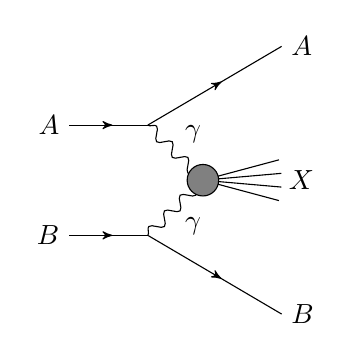
\begin{tikzpicture}[baseline=(baseline)]
    \coordinate (P1in)  at (-1.7,  0.7);
    \coordinate (V1)    at (-0.7,  0.7);
    \coordinate (P1out) at ( 1.0,  1.7);
    \coordinate (V)     at (   0,    0);
    \coordinate (P2in)  at (-1.7, -0.7);
    \coordinate (V2)    at (-0.7, -0.7);
    \coordinate (P2out) at ( 1.0, -1.7);

    \draw [fermion] (P1in) node [left] {$A$} -- (V1);
    \draw [fermion] (V1)   -- (P1out) node [right] {$A$};
    \draw [fermion] (P2in) node [left] {$B$} -- (V2);
    \draw [fermion] (V2)   -- (P2out) node [right] {$B$};
    \draw [photon]  (V1)   -- node [above right] {$\gamma$} (V);
    \draw [photon]  (V2)   -- node [below right] {$\gamma$} (V);

    \draw (V) -- +( 15:1);
    \draw (V) -- +(  5:1);
    \draw (V) -- +( -5:1);
    \draw (V) -- +(-15:1);

    \node at (1.25, 0) {$X$};

    \draw [fill=gray] (V) circle (0.2);

    \coordinate (baseline) at ([yshift=-0.5ex]current bounding box.center);
  \end{tikzpicture}
  \caption{Feynman diagram of an ultraperipheral collision $AB \to ABX$.}
  \label{f:upc}
\end{figure}
Differential cross section for the process $AB \to ABX$ (see fig.~\ref{f:upc})
with non-electromagnetic interactions neglected:
\begin{equation}
  \frac{\mathrm{d} \sigma(AB \to ABX)}{\mathrm{d} \sqrt{s}}
  = \sigma(\gamma \gamma \to X) \, \frac{\mathrm{d} L}{\mathrm{d} \sqrt{s}},
\end{equation}
where $\sigma(\gamma \gamma \to X)$ is the cross section for the fusion of two
(real) photons to a system $X$.

Differential cross section for the process $AB \to ABX$ with non-electromagnetic
interactions respected:
\begin{equation}
  \frac{\mathrm{d} \sigma(AB \to ABX)}{\mathrm{d} \sqrt{s}}
  = \sigma_\parallel(\gamma \gamma \to X)
    \, \frac{\mathrm{d} L_\parallel}{\mathrm{d} \sqrt{s}}
  + \sigma_\perp(\gamma \gamma \to X)
    \, \frac{\mathrm{d} L_\perp}{\mathrm{d} \sqrt{s}},
\end{equation}
where $\sigma_{\parallel,\perp}(\gamma \gamma \to X)$ are the cross sections for
the fusion of two photons with parallel or perpendicular polarizations,
$L_{\parallel,\perp}$ are photon-photon luminosities with respect to photon
polarizations.

Differential fiducial cross section for the process $AB \to AB \chi^+ \chi^-$
with the non-electromagnetic interactions neglected and with the constraints on
the phase space $p_T^\pm > \hat p_T$, $\abs{\eta^\pm} < \hat \eta$, $\omega_{1,
\text{min}} < \omega_1 < \omega_{1, \text{max}}$, $\omega_{2, \text{min}} <
\omega_2 < \omega_{2, \text{max}}$, where $p_T^\pm$ and $\eta^\pm$ are the
transverse momentum and pseudorapidity of $\chi^\pm$, and $\omega_{1,
\text{min}}$, $\omega_{1, \text{max}}$, $\omega_{2, \text{min}}$, $\omega_{2,
\text{max}}$ are the limits on the photon energies:\footnote{The third argument
to $\max$ in~\eqref{pt-min} currently neglects the mass of $\chi$. To be
updated.}
\begin{gather}
  \frac{\mathrm{d} \sigma_\text{fid.}(AB \to AB \chi^+ \chi^-)}
       {\mathrm{d} \sqrt{s}}
  = \int\limits_{\tilde p_T}
               ^{\frac{\sqrt{s}}{2} \sqrt{1 - \frac{4 m_\chi^2}{s}}}
      \mathrm{d} p_T
      \, \frac{\mathrm{d} \sigma(\gamma \gamma \to \chi^+ \chi^-)}
              {\mathrm{d} p_T}
      \, \frac{\mathrm{d} \hat L}{\mathrm{d} \sqrt{s}},
  \\
  \frac{\mathrm{d} \hat L}{\mathrm{d} \sqrt{s}}
  = \frac{\sqrt{s}}{2}
    \int\limits_{\max(-\hat y, \tilde y)}^{\min(\hat y, \tilde Y)} \mathrm{d} y
    \, n \left( \frac{\sqrt{s}}{2} \mathrm{e}^y \right)
    \, n \left( \frac{\sqrt{s}}{2} \mathrm{e}^{-y} \right),
  \\
  \hat y = \arcsinh \left[
    \frac{p_T \sqrt{s}}{2 (p_T^2 + m_\chi^2)} \left(
      \sinh \hat \eta
      - \sqrt{\cosh^2 \hat \eta + \frac{m_\chi^2}{p_T^2}}
        \cdot \sqrt{1 - \frac{4 (p_T^2 + m_\chi^2)}{s}}
    \right)
  \right],
  \\
  \tilde p_T
  = \max \left(
      \hat p_T,
      \frac{\sqrt{s}}{2 \cosh \hat \eta} \sqrt{1 - \frac{4 m_\chi^2}{s}},
      \frac{\sqrt{s}}{2 \cosh(\max(\tilde y, -\tilde Y) - \hat \eta)}
    \right),
    \label{pt-min}
  \\
  \begin{aligned}
    \\
    \tilde y
    &= \ln \max \left(
         \frac{2 \omega_{1, \text{min}}}{s}, \frac{s}{2 \omega_{2, \text{max}}}
       \right),
    \\
    \tilde Y
    &= \ln \max \left(
         \frac{2 \omega_{1, \text{max}}}{s}, \frac{s}{2 \omega_{2, \text{min}}}
       \right).
  \end{aligned}
\end{gather}

Differential fiducial cross section for the process $AB \to AB \chi^+ \chi^-$
with the non-electromagnetic interactions respected and with the constraints on
the phase space $p_T^\pm > \hat p_T$, $\abs{\eta^\pm} < \hat \eta$, where
$p_T^\pm$ and $\eta^\pm$ are the transverse momentum and pseudorapidity of
$\chi^\pm$:
\begin{gather}
  \begin{multlined}
    \frac{\mathrm{d} \sigma_\text{fid.}(AB \to AB \chi^+ \chi^-)}
         {\mathrm{d} \sqrt{s}}
    = \\ \int\limits_{\tilde p_T}
                    ^{\frac{\sqrt{s}}{2} \sqrt{1 - \frac{4 m_\chi^2}{s}}}
        \mathrm{d} p_T
        \left(
            \frac{\mathrm{d} \sigma_\parallel(\gamma \gamma \to \chi^+ \chi^-)}
                 {\mathrm{d} p_T}
            \frac{\mathrm{d} \hat L_\parallel}{\mathrm{d} \sqrt{s}}
          + \frac{\mathrm{d} \sigma_\perp(\gamma \gamma \to \chi^+ \chi^-)}
                 {\mathrm{d} p_T}
            \frac{\mathrm{d} \hat L_\perp}{\mathrm{d} \sqrt{s}}
        \right),
  \end{multlined}
  \\
  \frac{\mathrm{d} \hat L_\parallel}{\mathrm{d} \sqrt{s}}
  = \frac{\sqrt{s}}{2}
    \iint \mathrm{d}^2 b_1 \mathrm{d}^2 b_2 P(b)
    \int\limits_{-\hat y}^{\hat y} \mathrm{d} y
    \, n \left( b_1, \frac{\sqrt{s}}{2} \mathrm{e}^y    \right)
    \, n \left( b_2, \frac{\sqrt{s}}{2} \mathrm{e}^{-y} \right)
    \cos^2 \varphi
  \\
  \frac{\mathrm{d} \hat L_\perp}{\mathrm{d} \sqrt{s}}
  = \frac{\sqrt{s}}{2}
    \iint \mathrm{d}^2 b_1 \mathrm{d}^2 b_2 P(b)
    \int\limits_{-\hat y}^{\hat y} \mathrm{d} y
    \, n \left( b_1, \frac{\sqrt{s}}{2} \mathrm{e}^y    \right)
    \, n \left( b_2, \frac{\sqrt{s}}{2} \mathrm{e}^{-y} \right)
    \sin^2 \varphi
\end{gather}

\section{Proton}

Proton current:
\begin{equation}
  \bar u(p_2) \left[
    F_1(Q^2) \gamma_\mu - F_2(Q^2) \frac{\sigma_{\mu \nu} q^\nu}{2 m_p}
  \right] u(p_1),
  \ 
  \sigma_{\mu \nu} = \frac12 ( \gamma_\mu \gamma_\nu - \gamma_\nu \gamma_\mu).
\end{equation}

Proton form factors: \\
\begin{center}
  \begin{tabular}{rl}
    electric
    & $G_E(Q^2) = \frac{1}{\left(1 + \frac{Q^2}{\Lambda^2} \right)^2}$, \\
    magnetic
    & $G_M(Q^2) = \frac{\mu_p}{\left(1 + \frac{Q^2}{\Lambda^2} \right)^2}$, \\
    Dirac
    &
    $F_1(Q^2)
     = \frac{G_E(Q^2) + \frac{Q^2}{4 m_p^2} G_M(Q^2)}
            {1 + \frac{Q^2}{4 m_p^2}}$, \\
    Pauli
    & $F_2(Q^2) = \frac{G_M(Q^2) - G_E(Q^2)}{1 + \frac{Q^2}{4 m_p^2}}$, \\
  \end{tabular}
\end{center}
where $\mu_p$ is the proton magnetic moment (ratio to nuclear magneton).

Equivalent photon spectrum of a proton (cf.~\eqref{spectrum}):
\begin{equation}
  n_p(\omega)
  = \frac{2 \alpha}{\pi \omega}
    \int\limits_0^\infty
      \frac{D(q_\perp^2 + (\omega / \gamma)^2)}
           {(q_\perp^2 + (\omega / \gamma)^2)^2}
      q_\perp^3
    \, \mathrm{d} q_\perp,
\end{equation}
where
\begin{equation}
  D(Q^2)
  = \frac{G_E^2(Q^2) + \frac{Q^2}{4 m_p^2} G_M^2(Q^2)}{1 + \frac{Q^2}{4 m_p^2}}.
\end{equation}

Equivalent photon spectrum of a proton with the form factor approximated with
the dipole formula:
\begin{multline}
  n_p(\omega)
  = \frac{\alpha}{\pi \omega}
    \left\{
      \left( 1 + 4 u - (\mu_p^2 - 1) \frac{u}{v} \right)
      \ln \left( 1 + \frac{1}{u} \right)
      - \frac{24 u^2 + 42 u + 17}{6 (u + 1)^2}
    \right. \\ \left.
      - \frac{\mu_p^2 - 1}{(v - 1)^3}
        \left[
            \frac{1 + u / v}{v - 1} \ln \frac{u + v}{u + 1}
          - \frac{6 u^2 (v^2 - 3v + 3) + 3u (3v^2 - 9v + 10) + 2v^2 - 7v + 11}
                 {6 (u + 1)^2}
        \right]
    \right\},
\end{multline}
where
\begin{equation}
  u = \left( \frac{\omega}{\Lambda \gamma} \right), \ 
  v = \left( \frac{2 m_p}{\Lambda} \right)^2.
\end{equation}

Equivalent photon spectrum of a proton with only the Dirac $(\psi \gamma_\mu
\psi)$ current taken into account and the form factor approximated with the
dipole formula (Eq.~\eqref{spectrum} with $F(Q^2) \equiv F_1(Q^2)$):
\begin{align*}
%  \begin{split}
   &n_{p, \text{Dirac}}(\omega)
    = \frac{\alpha}{\pi \omega}
      \left\{
          \left( 1 + 4 a - 2 (\mu - 1) \frac{a}{b} \right)
          \ln\left( 1 + \frac{1}{a} \right)
   \right. \\ &\qquad \left. {}
        + \frac{\mu - 1}{(b - 1)^4}
          \left(
            \frac{\mu - 1}{b - 1} (1 + 4 a + 3 b) - 2 \left( 1 + \frac{a}{b} \right)
          \right)
          \ln \frac{a + b}{a + 1}
        - \left( 4 + \frac{1}{a + 1} + \frac{1}{6 (a + 1)^2} \right)
   \right. \\ &\qquad \left. {}
        + 2 (\mu - 1) \left[
              \left( \frac{a}{b} + \frac{1 + a/b}{(b - 1)^3} \right)
              \frac{1}{a + 1}
            + \frac12
              \left( \frac{a}{b} - \frac{1 + a/b}{(b - 1)^2} \right)
              \frac{1}{(a + 1)^2}
            + \frac13
              \left( \frac{a}{b} + \frac{1 + a/b}{b - 1} \right)
              \frac{1}{(a + 1)^3}
         \right]
   \right. \\ &\qquad \left. {}
       - (\mu - 1)^2
         \left[
           \frac{1}{(b - 1)^4}
           + \frac{1 + 3 a + 2 b}{(a + 1) (b - 1)^4}
           - \frac{1 + 2 a + b}{2 (a + 1)^2 (b - 1)^3}
           + \frac{1}{3 (a + 1)^2 (b - 1)^2}
         \right]
     \right\}
    \\
    &= \frac{\alpha}{\pi \omega}
       \left\{
           \left( 1 + 4 u - 2 (\mu_p - 1) \frac{u}{v} \right)
           \ln \left( 1 + \frac{1}{u} \right)
    \right. \\ &\qquad \left. {}
         + \frac{\mu_p - 1}{(v - 1)^4} \left[
               \frac{\mu_p - 1}{v - 1} (1 + 4 u + 3 v)
             - 2 \left( 1 + \frac{u}{v} \right)
           \right]
           \ln \frac{u + v}{u + 1}
         - \frac{24 u^2 + 42 u + 17}{6 (u + 1)^2}
    \right. \\ &\qquad \left. {}
         + (\mu_p - 1) \,
           \frac{
             6 u^2 (v^2 - 3 v + 3) + 3 u (3 v^2 - 9 v + 10) + 2 v^2 - 7 v + 11
           }{
             3 (u + 1)^2 (v - 1)^3
           }
    \right. \\ &\qquad \left. {}
         - (\mu_p - 1)^2 \,
           \frac{
             24 u^2 + 6 u (v + 7) - v^2 + 8 v + 17
           }{
             6 (u + 1)^2 (v - 1)^4
           }
       \right\}.
    \stepcounter{equation}
    \tag{\theequation}
    \\
%  \end{split}
\end{align*}

Equivalent photon spectrum of a proton with only the Dirac $(\psi \gamma_\mu
\psi)$ current taken into account and the form factor approximated with the
dipole formula (Eq.~\eqref{spectrum} with $F(Q^2) \equiv F_1(Q^2)$):
\begin{equation}
  \begin{split}
    n_{p, \text{Dirac}}(b, \omega)
    &= \frac{\alpha}{\pi^2 \omega}
       \left[
           \frac{\omega}{\gamma} K_1 \left( \frac{b \omega}{\gamma} \right)
         - \left(
               1
             + \frac{(\mu_p - 1) \frac{\Lambda^4}{16 m_p^4}}{
                 \left( 1 - \frac{\Lambda^2}{4 m_p^2} \right)^2
               }
           \right)
           \sqrt{\Lambda^2 + \frac{\omega^2}{\gamma^2}}
           \, K_1 \left( b \sqrt{\Lambda^2 + \frac{\omega^2}{\gamma^2}} \right)
    \right. \\ &\qquad \left.
         + \frac{(\mu_p - 1) \frac{\Lambda^4}{16 m_p^4}}{
             \left( 1 - \frac{\Lambda^2}{4 m_p^2}  \right)^2
           }
           \sqrt{4 m_p^2 + \frac{\omega^2}{\gamma^2}}
           \, K_1 \left( b \sqrt{4 m_p^2 + \frac{\omega^2}{\gamma^2}} \right)
    \right. \\ &\qquad \left.
         - \frac{1 - \frac{\mu_p \Lambda^2}{4 m_p^2}}
                {1 - \frac{\Lambda^2}{4 m_p^2}}
         \cdot
           \frac{b \Lambda^2}{2}
           \, K_0 \left( b \sqrt{\Lambda^2 + \frac{\omega^2}{\gamma^2}} \right)
       \right]^2.
  \end{split}
\end{equation}

Empirical formula for the probability to avoid non-electromagnetic interactions
in an ultraperipheral collision of two protons~\cite{hep-ph-0608271}:
\begin{equation}
  P(b) = \left( 1 - \mathrm{e}^{-\frac{b^2}{2B}} \right)^2,
\end{equation}
where~\cite{1112.3243}
\begin{equation}
  B = B_0 + 2 B_1 \ln(E / E_0) + 4 B_2 \ln^2 (E / E_0),
\end{equation}
$B_0 = 12~\text{GeV}^{-2}$, $B_1 = -0.22 \pm 0.17~\text{GeV}^2$, $B_2 = 0.037
\pm 0.006~\text{GeV}^{-2}$, $E$ is the collision energy, $E_0 = 1$~GeV.

Photon-photon luminosity in an ultraperipheral collison of two protons:
\begin{equation}
  \begin{gathered}
    \begin{multlined}
      \frac{\mathrm{d} L_\parallel}{\mathrm{d} \sqrt{s}}
      = \pi^2 \sqrt{s}
        \int\limits_0^\infty b_1 \, \mathrm{d} b_1
        \int\limits_0^\infty b_2 \, \mathrm{d} b_2
        \int\limits_{-\infty}^\infty \mathrm{d} y
        \, n \left( b_1, \tfrac{\sqrt{s}}{2} \, \mathrm{e}^y \right)
        \, n \left( b_2, \tfrac{\sqrt{s}}{2} \, \mathrm{e}^{-y} \right)
        \\  \times
        \left\{
            1
          - 2 \mathrm{e}^{-\frac{b_1^2 + b_2^2}{2 B}}
            \left[
                I_0 \left( \frac{b_1 b_2}{B} \right)
              + I_2 \left( \frac{b_1 b_2}{B} \right)
            \right]
          + \mathrm{e}^{-\frac{b_1^2 + b_2^2}{B}}
            \left[
                I_0 \left( \frac{2 b_1 b_2}{B} \right)
              + I_2 \left( \frac{2 b_1 b_2}{B} \right)
            \right]
        \right\},
    \end{multlined}
    \\
    \begin{multlined}
      \frac{\mathrm{d} L_\perp}{\mathrm{d} \sqrt{s}}
      = \pi^2 \sqrt{s}
        \int\limits_0^\infty b_1 \, \mathrm{d} b_1
        \int\limits_0^\infty b_2 \, \mathrm{d} b_2
        \int\limits_{-\infty}^\infty \mathrm{d} y
        \, n \left( b_1, \tfrac{\sqrt{s}}{2} \, \mathrm{e}^y \right)
        \, n \left( b_2, \tfrac{\sqrt{s}}{2} \, \mathrm{e}^{-y} \right)
        \\  \times
        \left\{
            1
          - 2 \mathrm{e}^{-\frac{b_1^2 + b_2^2}{2 B}}
            \left[
                I_0 \left( \frac{b_1 b_2}{B} \right)
              - I_2 \left( \frac{b_1 b_2}{B} \right)
            \right]
          + \mathrm{e}^{-\frac{b_1^2 + b_2^2}{B}}
            \left[
                I_0 \left( \frac{2 b_1 b_2}{B} \right)
              - I_2 \left( \frac{2 b_1 b_2}{B} \right)
            \right]
        \right\},
    \end{multlined}
  \end{gathered}
\end{equation}
where $I_0(x)$, $I_2(x)$ are the modified Bessel function of the first kind.

\section{Fermion pair production}

Breit-Wheeler cross sections for fermion pair production in photon-photon
collisions:
\begin{gather}
    \sigma_\parallel(\gamma \gamma \to \chi^+ \chi^-)
    = \frac{4 \pi \alpha^2}{s}
      \left[
        \left( 1 + \frac{4 m_\chi^2}{s} - \frac{12 m_\chi^4}{s^2} \right)
        \ln \frac{1 + \sqrt{1 - 4 m_\chi^2 / s}}
                 {1 - \sqrt{1 - 4 m_\chi^2 / s}}
        - \left( 1 + \frac{6 m_\chi^2}{s} \right)
          \sqrt{1 - \frac{4 m_\chi^2}{s}}
      \right],
    \\
    \sigma_\perp(\gamma \gamma \to \chi^+ \chi^-)
    = \frac{4 \pi \alpha^2}{s}
      \left[
        \left( 1 + \frac{4 m_\chi^2}{s} - \frac{4 m_\chi^4}{s^2} \right)
        \ln \frac{1 + \sqrt{1 - 4 m_\chi^2 / s}}
                 {1 - \sqrt{1 - 4 m_\chi^2 / s}}
        - \left( 1 + \frac{2 m_\chi^2}{s} \right)
          \sqrt{1 - \frac{4 m_\chi^2}{s}}
      \right],
    \\
    \sigma(\gamma \gamma \to \chi^+ \chi^-)
    = \frac{4 \pi \alpha^2}{s}
      \left[
        \left( 1 + \frac{4 m_\chi^2}{s} - \frac{8 m_\chi^2}{s} \right)
        \ln \frac{1 + \sqrt{1 - 4 m_\chi^2 / s}}
                 {1 - \sqrt{1 - 4 m_\chi^2 / s}}
        - \left( 1 + \frac{4 m_\chi^2}{s} \right)
          \sqrt{1 - \frac{4 m_\chi^2}{s}}
     \right].
\end{gather}

Differential cross section with respect to the transverse momentum of the
fermions, $p_T$:
\begin{gather}
  \frac{\mathrm{d} \sigma_\parallel(\gamma \gamma \to \chi^+ \chi^-)}
       {\mathrm{d} p_T}
  = \frac{8 \pi \alpha^2 p_T}{s (p_T^2 + m_\chi^2)}
    \cdot \frac{1 - \frac{2 (p_T^4 + 2 m_\chi^4)}{s (p_T^2 + m_\chi^2)}}
               {\sqrt{1 - \frac{4 (p_T^2 + m_\chi^2)}{s}}},
  \\
  \frac{\mathrm{d} \sigma_\perp(\gamma \gamma \to \chi^+ \chi^-)}
       {\mathrm{d} p_T}
  = \frac{8 \pi \alpha^2 p_T}{s (p_T^2 + m_\chi^2)}
    \cdot \frac{1 - \frac{2 p_T^4}{s (p_T^2 + m_\chi^2)}}
               {\sqrt{1 - \frac{4 (p_T^2 + m_\chi^2)}{s}}},
  \\
  \frac{\mathrm{d} \sigma(\gamma \gamma \to \chi^+ \chi^-)}
       {\mathrm{d} p_T}
  = \frac{8 \pi \alpha^2 p_T}{s (p_T^2 + m_\chi^2)}
    \cdot \frac{1 - \frac{2 (p_T^4 + m_\chi^4)}{s (p_T^2 + m_\chi^2)}}
               {\sqrt{1 - \frac{4 (p_T^2 + m_\chi^2)}{s}}}.
\end{gather}

\newcommand{\arxiv}[1]{\href{http://arxiv.org/abs/#1}{arXiv:\nolinebreak[3]#1}}
\begin{thebibliography}{99}
  \bibitem{hep-ph-0608271}
  L.~Frankfurt, C.~E.~Hyde-Wright, M.~Strikman, C.~Weiss.
  Generalized parton distributions and rapidity gap survival in exclusive diffractive $p p$ scattering.
  Phys.Rev.~D75, 054009 (2007).
  \href{http://arxiv.org/abs/hep-ph/0608271}{arXiv:\nolinebreak[3]hep-ph/0608271}

  \bibitem{1112.3243}
  V.~A.~Schegelsky, M.~G.~Ryskin.
  Diffraction cone shrinkage speed up with the collision energy.
  Phys.Rev.~D85, 094024 (2012).
  \arxiv{1112.3243}
\end{thebibliography}



\end{document}
